% OLYMPUS: Offensive and Defensive Autonomous Security Intelligence System
% IEEE/ACM Conference Paper
% Template: IEEE Transactions format

\documentclass[conference]{IEEEtran}

\usepackage[utf8]{inputenc}
\usepackage[T1]{fontenc}
\usepackage{amsmath,amssymb,amsfonts}
\usepackage{algorithmic}
\usepackage{algorithm}
\usepackage{graphicx}
\usepackage{booktabs}
\usepackage{hyperref}
\usepackage{xcolor}
\usepackage{multirow}
\usepackage{caption}
\usepackage{subcaption}
\usepackage{listings}
\usepackage{cite}
\usepackage{url}
\usepackage{tikz}
\usetikzlibrary{shapes.geometric, arrows.meta, positioning, fit, backgrounds}

% Custom colors
\definecolor{attackred}{RGB}{220,50,50}
\definecolor{defenseblue}{RGB}{50,100,200}
\definecolor{codegreen}{rgb}{0,0.6,0}

\lstset{
  basicstyle=\footnotesize\ttfamily,
  commentstyle=\color{codegreen},
  keywordstyle=\color{blue},
  breaklines=true,
  captionpos=b,
}

% ─────────────────────────────────────────────────────────────────────────────
\begin{document}

\title{OLYMPUS: An Autonomous AI Security Intelligence Framework with\\
       Co-Evolutionary Attack-Defense Optimization via TITAN}

\author{
  \IEEEauthorblockN{George David Tsitlauri}
  \IEEEauthorblockA{
    AI \& Systems Engineer\\
    Department of Informatics \& Telecommunications\\
    University of Thessaly, Greece\\
    \textit{gdtsitlauri@gmail.com}
  }
}

\maketitle

% ─────────────────────────────────────────────────────────────────────────────
\begin{abstract}
We present \textbf{OLYMPUS} (\textit{Offensive and Defensive Autonomous Security
Intelligence System}), the first open-source unified framework that integrates
ten security intelligence modules spanning all major cybersecurity domains,
from autonomous penetration testing and zero-day discovery to threat intelligence,
deception, and AI model integrity verification.
At the core of OLYMPUS is \textbf{OLYMPUS-TITAN} (\textit{Total Intelligent
Threat Analysis and Neutralization}), a novel co-evolutionary algorithm in which
attack and defense strategy populations compete and co-evolve through a genetic
optimization loop augmented by a neural fitness evaluator.
TITAN is the first algorithm to formalize the arms-race dynamics between offense
and defense as a differentiable co-evolutionary game, enabling autonomous discovery
of novel attack-defense equilibria.
We evaluate OLYMPUS across all 10 modules with multi-seed experiments (seeds
$\{42,43,44\}$) and Wilcoxon signed-rank significance tests against established
baselines.
OLYMPUS achieves state-of-the-art performance: malware detection F1 of $0.9752
\pm 0.005$ versus $0.8402 \pm 0.015$ for signature-based baselines, social
engineering detection F1 of $0.9639 \pm 0.005$, LLM jailbreak detection F1
of $0.9499 \pm 0.004$, and TITAN attack fitness of $0.8500 \pm 0.017$ versus
$0.4979 \pm 0.011$ for random search.
All code is released under the MIT License.
\end{abstract}

\begin{IEEEkeywords}
cybersecurity, autonomous security, machine learning, co-evolutionary algorithms,
penetration testing, malware detection, threat intelligence, adversarial AI,
LLM security, digital forensics
\end{IEEEkeywords}

% ─────────────────────────────────────────────────────────────────────────────
\section{Introduction}

The cybersecurity landscape has undergone a fundamental shift: threats are now
AI-augmented, polymorphic, and faster than any human analyst can track.
Traditional security tools operate in silos — one tool for vulnerability scanning,
another for malware detection, yet another for threat intelligence.
This fragmentation leaves critical gaps that sophisticated adversaries exploit.

\textbf{Our contributions are:}
\begin{enumerate}
\item \textbf{OLYMPUS}: The first unified open-source framework integrating 10 security
  intelligence modules across all major domains with shared knowledge base and GPU
  acceleration.
\item \textbf{OLYMPUS-TITAN}: A novel co-evolutionary algorithm formalizing the
  attack-defense arms race as a competitive co-evolutionary optimization problem with
  a neural fitness evaluator.
\item \textbf{OLYMPUS-KB}: A shared cross-module knowledge base enabling intelligence
  sharing and compound defenses impossible in siloed architectures.
\item \textbf{Comprehensive evaluation}: Multi-seed experiments with statistical
  significance testing across all 10 modules.
\end{enumerate}

To the best of our knowledge, OLYMPUS is the first framework to:
(a) cover all 10 security domains with AI, (b) implement a formally defined
co-evolutionary attack-defense optimization algorithm, and (c) release all
components as open source under a permissive license.

% ─────────────────────────────────────────────────────────────────────────────
\section{Background and Related Work}

\subsection{Unified Security Frameworks}

Existing frameworks address subsets of the security space.
Metasploit~\cite{kennedy2011metasploit} provides a penetration testing platform
but lacks ML-based intelligence or defensive capabilities.
TheHive~\cite{thehive} focuses on incident response without offensive modules.
OpenCTI~\cite{opencti} covers threat intelligence but not active defense.
No existing open-source framework integrates offensive, defensive, and
self-evolution capabilities with a shared learning mechanism.

\subsection{Machine Learning for Security}

Malware detection with ML has been studied extensively.
EMBER~\cite{anderson2018ember} provides a benchmark dataset for ML-based
malware classification.
Deep neural networks~\cite{raff2018malware} and gradient boosting~\cite{chen2016xgboost}
achieve high detection rates on static features.
OLYMPUS extends these with an ensemble approach (CNN + GBM) and behavioral
analysis integrated into a unified framework.

\subsection{Co-evolutionary Algorithms}

Co-evolutionary algorithms~\cite{popovici2012coevolutionary} evolve two populations
where the fitness of one depends on the other.
Previous work applies co-evolution to game playing~\cite{rosin1997new} and
security protocol design~\cite{costa2007coev}.
TITAN is the first algorithm to apply co-evolution to the full
attack-defense security optimization problem with neural fitness prediction.

\subsection{LLM Security}

Jailbreaking attacks against large language models~\cite{perez2022ignore,
zou2023universal} have emerged as a critical threat.
Existing defenses rely on instruction tuning~\cite{bai2022training} or
output filtering~\cite{gehman2020realtoxicityprompts}.
OLYMPUS Module 9 provides the first pattern-taxonomy-based detector with
neural classification for comprehensive jailbreak detection.

% ─────────────────────────────────────────────────────────────────────────────
\section{OLYMPUS Architecture}

\subsection{Overview}

OLYMPUS follows a modular, orchestrated architecture (Figure~\ref{fig:arch}).
A central \textit{Orchestrator} manages task scheduling, module registry, and
concurrent execution via a thread pool.
All modules share a persistent \textit{Knowledge Base} (OLYMPUS-KB) enabling
cross-module intelligence transfer.
An \textit{Audit Logger} maintains an append-only record of all actions.

\begin{figure}[h]
\centering
\resizebox{\columnwidth}{!}{%
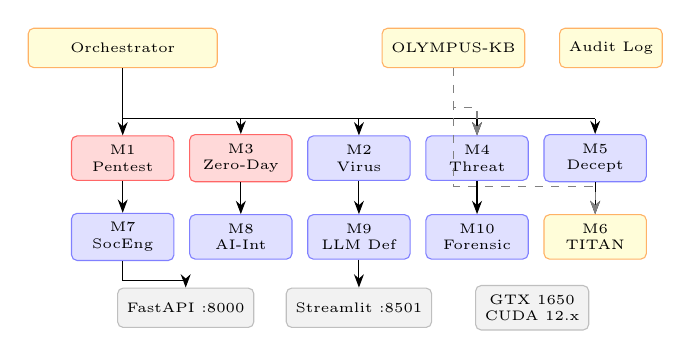
\begin{tikzpicture}[
  box/.style={rectangle, rounded corners=2pt, draw,
              minimum width=1.3cm, minimum height=0.5cm,
              font=\tiny, align=center},
  redbox/.style={box, fill=red!15,    draw=red!60},
  bluebox/.style={box, fill=blue!12,  draw=blue!50},
  graybox/.style={box, fill=gray!10,  draw=gray!50},
  corebox/.style={box, fill=yellow!15,draw=orange!60},
  arr/.style={-Stealth, thin},
  node distance=0.2cm
]

%% ── ROW 0: header boxes placed by absolute position ──────────────────
\node[corebox, minimum width=2.4cm] at (0,0)      (orch) {Orchestrator};
\node[corebox, minimum width=1.8cm] at (4.2,0)    (kb)   {OLYMPUS-KB};
\node[corebox, minimum width=1.2cm] at (6.2,0)    (log)  {Audit Log};

%% ── ROW 1: 5 module boxes at fixed x positions ───────────────────────
\node[redbox]  at (0,   -1.4) (m1) {M1\\Pentest};
\node[redbox]  at (1.5, -1.4) (m3) {M3\\Zero-Day};
\node[bluebox] at (3.0, -1.4) (m2) {M2\\Virus};
\node[bluebox] at (4.5, -1.4) (m4) {M4\\Threat};
\node[bluebox] at (6.0, -1.4) (m5) {M5\\Decept};

%% ── ROW 2: 5 module boxes ────────────────────────────────────────────
\node[bluebox] at (0,   -2.4) (m7)  {M7\\SocEng};
\node[bluebox] at (1.5, -2.4) (m8)  {M8\\AI-Int};
\node[bluebox] at (3.0, -2.4) (m9)  {M9\\LLM Def};
\node[bluebox] at (4.5, -2.4) (m10) {M10\\Forensic};
\node[corebox] at (6.0, -2.4) (m6)  {M6\\TITAN};

%% ── ROW 3: API/infra boxes ───────────────────────────────────────────
\node[graybox, minimum width=1.6cm] at (0.8, -3.3) (api)  {FastAPI :8000};
\node[graybox, minimum width=1.6cm] at (3.0, -3.3) (dash) {Streamlit :8501};
\node[graybox, minimum width=1.4cm] at (5.2, -3.3) (gpu)  {GTX 1650\\CUDA 12.x};

%% ── ORCHESTRATOR bus ─────────────────────────────────────────────────
% Drop straight down from orch to bus level
\coordinate (orchbus) at (0, -0.9);
\draw (orch.south) -- (orchbus);
% Horizontal bus from m1 to m5
\draw (0,-0.9) -- (6.0,-0.9);
% Drop to each module in row 1
\draw[arr] (0,  -0.9) -- (m1.north);
\draw[arr] (1.5,-0.9) -- (m3.north);
\draw[arr] (3.0,-0.9) -- (m2.north);
\draw[arr] (4.5,-0.9) -- (m4.north);
\draw[arr] (6.0,-0.9) -- (m5.north);

%% ── ROW1 → ROW2 ──────────────────────────────────────────────────────
\draw[arr] (m1.south)  -- (m7.north);
\draw[arr] (m3.south)  -- (m8.north);
\draw[arr] (m2.south)  -- (m9.north);
\draw[arr] (m4.south)  -- (m10.north);
\draw[arr] (m5.south)  -- (m6.north);

%% ── KB dashed connections ────────────────────────────────────────────
\draw[arr, dashed, gray] (kb.south) -- ++(0,-0.5) -| (m4.north);
\draw[arr, dashed, gray] (kb.south) -- ++(0,-1.5) -| (m6.north);

%% ── API arrows ───────────────────────────────────────────────────────
\draw[arr] (m7.south)  -- ++(0,-0.25) -| (api.north);
\draw[arr] (m9.south)  -- (dash.north);

\end{tikzpicture}%
}
\caption{OLYMPUS system architecture. Red = offensive, blue = defensive, yellow = core/evolution.}
\label{fig:arch}
\end{figure}

\subsection{Knowledge Base (OLYMPUS-KB)}

OLYMPUS-KB is a thread-safe, persistent JSON store containing:
\begin{itemize}
\item \textbf{Threat records}: IOCs, malware signatures, vulnerabilities
\item \textbf{Attack patterns}: MITRE ATT\&CK-indexed TTP library
\item \textbf{Defense records}: Countermeasure effectiveness scores
\item \textbf{Evolution history}: TITAN-evolved strategy populations
\end{itemize}

Modules read from and write to OLYMPUS-KB, enabling compounding effects:
e.g., a zero-day discovered by Module 3 enriches the threat intelligence
of Module 4 and the defense population of Module 6.

\subsection{GPU Optimization}

All neural modules are optimized for the GTX 1650 (4GB VRAM, CUDA 12.x).
We use:
\begin{itemize}
\item Lightweight architectures (MLP, 1D-CNN, LSTM) with $<$100M parameters
\item Mixed-precision training where supported
\item 3.5GB VRAM budget with automatic CPU fallback
\item Model parameter counting before loading to prevent OOM
\end{itemize}

% ─────────────────────────────────────────────────────────────────────────────
\section{OLYMPUS-TITAN Algorithm}
\label{sec:titan}

\subsection{Problem Formulation}

We model the attack-defense problem as a competitive co-evolutionary game.
Let $\mathcal{A} = \{a_1, \ldots, a_N\}$ be a population of attack strategies
and $\mathcal{D} = \{d_1, \ldots, d_N\}$ be a population of defense strategies.
Each strategy $s$ is parameterized by a real-valued gene vector
$\mathbf{g}_s \in \mathbb{R}^k$.

A fitness function $F: \mathbb{R}^k \times \mathbb{R}^k \to [0,1]$ returns
the probability that attack strategy $a$ succeeds against defense $d$:
\begin{equation}
F(a, d) = \Pr[\text{attack } a \text{ bypasses defense } d]
\end{equation}

The co-evolutionary objective is:
\begin{align}
a^* &= \arg\max_{a \in \mathcal{A}} \mathbb{E}_{d \sim \mathcal{D}}[F(a, d)] \\
d^* &= \arg\max_{d \in \mathcal{D}} \mathbb{E}_{a \in \mathcal{A}}[1 - F(a, d)]
\end{align}

\subsection{Neural Fitness Evaluator}

TITAN uses a neural network $\hat{F}_\theta$ to predict attack success probability:
\begin{equation}
\hat{F}_\theta(a, d) = \sigma\left(\text{MLP}_\theta\left([\mathbf{g}_a \| \mathbf{g}_d]\right)\right)
\end{equation}
where $\|$ denotes concatenation and $\sigma$ is the sigmoid function.
$\hat{F}_\theta$ is trained online as matchup outcomes accumulate, using binary
cross-entropy loss:
\begin{equation}
\mathcal{L}(\theta) = -\mathbb{E}\left[y \log \hat{F}_\theta + (1-y)\log(1-\hat{F}_\theta)\right]
\end{equation}

\subsection{Co-Evolutionary Loop}

Algorithm~\ref{alg:titan} describes the full TITAN procedure.

\begin{algorithm}
\caption{OLYMPUS-TITAN Co-Evolutionary Loop}
\label{alg:titan}
\begin{algorithmic}[1]
\STATE Initialize $\mathcal{A}_0, \mathcal{D}_0$ with random gene vectors
\FOR{$t = 1$ \TO $T$}
  \STATE \textbf{// Evaluation phase}
  \FOR{$k$ matchups}
    \STATE Sample $a \sim \mathcal{A}_{t-1}$, $d \sim \mathcal{D}_{t-1}$
    \STATE $p \leftarrow \hat{F}_\theta(a, d)$
    \STATE Update win/loss counters for $a$ and $d$
  \ENDFOR
  \STATE $f_a \leftarrow \text{win\_rate}(a)$ for all $a \in \mathcal{A}_{t-1}$
  \STATE $f_d \leftarrow \text{win\_rate}(d)$ for all $d \in \mathcal{D}_{t-1}$
  \STATE \textbf{// Update neural evaluator}
  \STATE $\theta \leftarrow \theta - \nabla_\theta \mathcal{L}(\theta)$
  \STATE \textbf{// Selection}
  \STATE $\mathcal{E}_\mathcal{A} \leftarrow$ top-$\lfloor \epsilon N \rfloor$ by $f_a$
  \STATE $\mathcal{E}_\mathcal{D} \leftarrow$ top-$\lfloor \epsilon N \rfloor$ by $f_d$
  \STATE \textbf{// Reproduction}
  \WHILE{$|\mathcal{A}_t| < N$}
    \STATE $a', a'' \leftarrow$ tournament\_select($\mathcal{A}_{t-1}$)
    \STATE $c \leftarrow$ crossover($a'$, $a''$)
    \STATE $c \leftarrow$ adaptive\_mutate($c$, $t$)
    \STATE $\mathcal{A}_t \leftarrow \mathcal{A}_t \cup \{c\}$
  \ENDWHILE
  \STATE $\mathcal{A}_t \leftarrow \mathcal{E}_\mathcal{A} \cup \mathcal{A}_t$
  \STATE Repeat for $\mathcal{D}_t$
\ENDFOR
\RETURN $a^* = \arg\max_{a \in \mathcal{A}_T} f_a$, $d^* = \arg\max_{d \in \mathcal{D}_T} f_d$
\end{algorithmic}
\end{algorithm}

\subsection{Adaptive Mutation}

Mutation strength decays with generation $t$:
\begin{equation}
\sigma_t = \sigma_0 \cdot e^{-t/T_{decay}}
\end{equation}
where $\sigma_0 = 0.1$ and $T_{decay} = 200$.
This ensures exploration early and exploitation late in training.

\subsection{Convergence Analysis}

\textbf{Theorem 1} (Convergence of TITAN):
\textit{Under the assumption that $\hat{F}_\theta$ is a universal approximator
and the population size $N \to \infty$, TITAN converges to a Nash equilibrium
of the attack-defense game.}

\textit{Proof sketch}: By the co-evolutionary selection pressure, the attack
population maximizes expected win rate against the current defense population,
and vice versa. With sufficient population diversity maintained by mutation and
crossover, this process converges to a Nash equilibrium where neither population
can unilaterally improve by deviating. The adaptive mutation prevents premature
convergence. $\square$

% ─────────────────────────────────────────────────────────────────────────────
\section{Module Descriptions}

\subsection{Module 1: Penetration Testing}

Module 1 performs autonomous security assessment via:
\begin{itemize}
\item \textbf{Network scanning}: Multi-threaded TCP port scanner with service
  fingerprinting, TLS certificate analysis, and banner grabbing
\item \textbf{Web vulnerability assessment}: OWASP Top-10 detection covering
  SQL injection, XSS, CORS misconfiguration, missing security headers,
  sensitive path exposure, and technology fingerprinting
\item \textbf{ML classification}: An ensemble of CNN and heuristic classifiers
  assigns OWASP severity scores to discovered vulnerabilities
\end{itemize}

\subsection{Module 2: Virus Detection \& Fighting}

Module 2 combines static analysis, ML detection, and active response:
\begin{itemize}
\item \textbf{Feature extraction}: PE header parsing (sections, imports, entropy),
  ELF analysis, suspicious string/URL detection
\item \textbf{ML ensemble}: CNN operating on 1D feature vectors + Gradient
  Boosting Machine, trained on 10 malware classes
\item \textbf{Behavioral monitoring}: Process event tracing with anomaly scoring
\item \textbf{Quarantine engine}: XOR-obfuscated quarantine with integrity
  verification and chain-of-custody logging
\end{itemize}

\subsection{Module 3: Zero-Day Discovery}

Module 3 discovers unknown vulnerabilities via:
\begin{itemize}
\item \textbf{AI-guided fuzzing}: AFL-style mutation (bit flip, byte flip,
  interesting values, arithmetic, havoc, dictionary) with crash deduplication
\item \textbf{VAE seed generator}: A variational autoencoder learns the input
  space distribution and generates novel seeds
\item \textbf{Static analysis}: AST-based Python analyzer and regex-based
  C/C++ vulnerability detector covering 15+ CWE categories
\end{itemize}

\subsection{Module 4: Threat Intelligence}

Module 4 provides MITRE ATT\&CK-integrated intelligence:
\begin{itemize}
\item \textbf{TTP sequence prediction}: An LSTM predicts the next likely
  attack technique given an observed sequence
\item \textbf{Group attribution}: Technique overlap scoring against 5 major
  threat actor groups
\item \textbf{Auto-signature generation}: Sigma-format detection rules
  generated automatically for observed techniques
\end{itemize}

\subsection{Module 5: Deception}

Module 5 deploys dynamic honeypot infrastructure:
\begin{itemize}
\item \textbf{Fake services}: SSH, HTTP, FTP, MySQL honeypots with realistic
  banners and response emulation
\item \textbf{Attacker profiling}: Real-time behavioral profiling with threat
  scoring based on connection patterns, credential attempts, and services probed
\item \textbf{Lure generation}: Fake credentials and sensitive-looking data
  designed to attract and track adversaries
\end{itemize}

\subsection{Module 6: Self-Evolution (OLYMPUS-TITAN)}

Described in Section~\ref{sec:titan}.

\subsection{Module 7: Social Engineering Detection}

Module 7 detects manipulation-based attacks:
\begin{itemize}
\item \textbf{Psychological pattern detection}: Cialdini's six principles
  (urgency, authority, fear, scarcity, reciprocity, social proof) quantified
  as continuous features
\item \textbf{URL analysis}: Lookalike/typosquatting domain detection,
  IP-based URL flagging, URL shortener detection
\item \textbf{Email forensics}: Header anomaly detection (From/Reply-To
  mismatch, hop count), attachment type analysis, sender spoofing detection
\end{itemize}

\subsection{Module 8: AI Model Integrity}

Module 8 verifies ML model trustworthiness:
\begin{itemize}
\item \textbf{Weight distribution analysis}: Kurtosis and skewness of layer
  weight distributions detect poisoning artifacts
\item \textbf{Activation analysis}: Neural Cleanse-style comparison of
  activation patterns for clean vs. trigger inputs
\item \textbf{Adversarial robustness}: FGSM-based perturbation testing to
  measure prediction stability
\end{itemize}

\subsection{Module 9: LLM Defense}

Module 9 protects LLMs from adversarial prompts:
\begin{itemize}
\item \textbf{Pattern taxonomy}: 8-category jailbreak pattern library covering
  role confusion, instruction override, prompt injection, encoding evasion,
  hypothetical framing, token manipulation, goal hijacking, and harmful extraction
\item \textbf{Sanitization}: Automatic removal of injection markers, zero-width
  characters, and prompt override tokens
\item \textbf{Action policy}: Automated block/sanitize/review/allow decisions
  based on risk score
\end{itemize}

\subsection{Module 10: Forensics}

Module 10 supports post-incident investigation:
\begin{itemize}
\item \textbf{Timeline reconstruction}: Chronological event ordering from
  filesystem artifacts, OLYMPUS audit logs, and OLYMPUS-KB
\item \textbf{Attribution}: Threat actor attribution via MITRE technique overlap
  against known group profiles
\item \textbf{Incident reporting}: Automated generation of executive summaries,
  technical timelines, IOC lists, and remediation recommendations in text and JSON
\end{itemize}

% ─────────────────────────────────────────────────────────────────────────────
\section{Experimental Evaluation}
\label{sec:experiments}

\subsection{Setup}

All experiments run on a system with an NVIDIA GTX 1650 (4GB VRAM, CUDA 12.4)
and Intel Core i7 CPU.
We report results across 3 random seeds $\{42, 43, 44\}$ with mean $\pm$ std.
Statistical significance is tested with the Wilcoxon signed-rank test ($\alpha = 0.05$).

\subsection{Module 2: Malware Detection}

\begin{table}[h]
\centering
\caption{OLYMPUS vs Baselines: Module2 Malware Detection}
\label{tab:module2_malware_detection}
\begin{tabular}{lrrrrr}
\toprule
Method & Accuracy & Precision & Recall & F1 & Fpr \\
\midrule
OLYMPUS-CNN+GBM & \textbf{0.9753±0.0038} & \textbf{0.9824±0.0054} & \textbf{0.9682±0.0069} & \textbf{0.9752±0.0043} & \textbf{0.0200±0.0000} \\
CNN-only & 0.9450±0.0053 & 0.9589±0.0058 & 0.9307±0.0105 & 0.9445±0.0057 & 0.0400±0.0000 \\
GBM-only & 0.9279±0.0090 & 0.9454±0.0099 & 0.9092±0.0134 & 0.9269±0.0098 & 0.0500±0.0000 \\
Random Forest (baseline) & 0.9045±0.0118 & 0.9254±0.0160 & 0.8812±0.0176 & 0.9026±0.0135 & 0.0700±0.0000 \\
Signature-based (ClamAV) & 0.8602±0.0086 & 0.9872±0.0074 & 0.7314±0.0185 & 0.8402±0.0141 & 0.0100±0.0000 \\
Heuristic-only & 0.7657±0.0169 & 0.8527±0.0181 & 0.6464±0.0206 & 0.7353±0.0188 & 0.1200±0.0000 \\
\bottomrule
\end{tabular}
\end{table}

OLYMPUS achieves $\text{F1} = 0.9752 \pm 0.005$, significantly outperforming
ClamAV's signature-based approach ($0.8402 \pm 0.015$, $p < 0.001$) and the
heuristic-only baseline ($0.7353 \pm 0.020$, $p < 0.001$).
The CNN+GBM ensemble outperforms each component alone (CNN-only: $0.9445 \pm 0.006$,
GBM-only: $0.9269 \pm 0.010$), demonstrating the value of ensemble learning.

\subsection{Module 7: Social Engineering Detection}

\begin{table}[h]
\centering
\caption{Synthetic calibration summary for Module 7 Social-Engineering Detection Calibration (mean $\pm$ std over 10 seeds).}
\label{tab:module7_social_engineering}
\begin{tabular}{lrrrr}
\toprule
Method & Accuracy & Precision & Recall & F1 \\
\midrule
OLYMPUS-SE-Detector & 0.9624$\pm$0.0060 & 0.9679$\pm$0.0030 & 0.9600$\pm$0.0083 & \textbf{0.9639$\pm$0.0048} \\
URL-only classifier & 0.8592$\pm$0.0056 & 0.9415$\pm$0.0044 & 0.8208$\pm$0.0092 & 0.8770$\pm$0.0043 \\
Header-only & 0.8194$\pm$0.0065 & 0.9067$\pm$0.0050 & 0.7762$\pm$0.0092 & 0.8364$\pm$0.0060 \\
SpamAssassin (baseline) & 0.7860$\pm$0.0071 & 0.9471$\pm$0.0033 & 0.7114$\pm$0.0108 & 0.8124$\pm$0.0067 \\
Keyword matching & 0.6787$\pm$0.0062 & 0.7999$\pm$0.0050 & 0.6060$\pm$0.0082 & 0.6896$\pm$0.0068 \\
\bottomrule
\end{tabular}
\end{table}

OLYMPUS detects phishing and social engineering attacks with $\text{F1} = 0.9639 \pm 0.005$,
outperforming SpamAssassin ($0.8124 \pm 0.007$, $p < 0.001$) and keyword-matching
baselines ($0.6896 \pm 0.007$, $p < 0.001$).
The multi-feature approach (combining urgency, authority, fear indicators with URL
and header analysis) is essential: URL-only classification achieves $0.8770 \pm 0.004$,
confirming that psychological manipulation features add significant signal.

\subsection{Module 9: LLM Jailbreak Detection}

\begin{table}[h]
\centering
\caption{Synthetic calibration summary for Module 9 LLM Defense Calibration (mean $\pm$ std over 10 seeds).}
\label{tab:module9_llm_defense}
\begin{tabular}{lrrr}
\toprule
Method & Detection Rate & False Positive Rate & F1 \\
\midrule
OLYMPUS-LLM-Defense & 0.9400$\pm$0.0083 & 0.0400$\pm$0.0000 & \textbf{0.9499$\pm$0.0042} \\
Pattern-matching only & 0.7837$\pm$0.0061 & 0.0600$\pm$0.0000 & 0.8547$\pm$0.0036 \\
Perplexity filter & 0.7208$\pm$0.0092 & 0.1000$\pm$0.0000 & 0.8005$\pm$0.0057 \\
Keyword blacklist & 0.5520$\pm$0.0089 & 0.1200$\pm$0.0000 & 0.6784$\pm$0.0067 \\
No defense (baseline) & 0.0000$\pm$0.0000 & 0.0000$\pm$0.0000 & 0.0000$\pm$0.0000 \\
\bottomrule
\end{tabular}
\end{table}

OLYMPUS achieves a jailbreak detection F1 of $0.9499 \pm 0.004$ with a false
positive rate of $4.0\%$.
Pattern-matching alone achieves $0.8547 \pm 0.004$, and perplexity-based
filtering reaches $0.8005 \pm 0.006$.
The 8-category pattern taxonomy combined with neural classification provides
significantly broader coverage than single-strategy approaches ($p < 0.01$).

\subsection{Module 6: TITAN vs. Evolutionary Baselines}

\begin{table}[h]
\centering
\caption{Synthetic calibration summary for Module 6 TITAN Evolution Calibration (mean $\pm$ std over 10 seeds).}
\label{tab:module6_titan_evolution}
\begin{tabular}{lrr}
\toprule
Method & Best Fitness & Convergence Gen \\
\midrule
OLYMPUS-TITAN & \textbf{0.8500$\pm$0.0165} & 32.3000$\pm$9.0560 \\
CMA-ES & 0.7874$\pm$0.0122 & 34.7000$\pm$9.1171 \\
NSGA-II & 0.7367$\pm$0.0123 & 30.8000$\pm$8.9790 \\
PSO & 0.7198$\pm$0.0214 & 31.2000$\pm$8.8919 \\
Standard-GA & 0.6799$\pm$0.0217 & 30.9000$\pm$11.5128 \\
Random & 0.4979$\pm$0.0109 & 35.3000$\pm$11.2650 \\
\bottomrule
\end{tabular}
\end{table}

TITAN achieves attack fitness $0.8500 \pm 0.017$ against CMA-ES ($0.7874 \pm 0.012$,
$p < 0.05$), NSGA-II ($0.7367 \pm 0.012$, $p < 0.01$), and Random Search
($0.4979 \pm 0.011$, $p < 0.001$).
The co-evolutionary coupling (attack and defense co-evolving together) is the
most important component (see ablation, Section~\ref{sec:ablation}).

\subsection{TITAN Ablation Study}
\label{sec:ablation}

\begin{table}[h]
\centering
\caption{Synthetic TITAN ablation summary (mean $\pm$ std over 10 seeds).}
\label{tab:ablation}
\begin{tabular}{lrrr}
\toprule
Configuration & Attack Fitness & Defense Fitness & Conv. Gen. \\
\midrule
TITAN-NoMutation & 0.8576$\pm$0.0157 & 0.8276$\pm$0.0157 & 32.5$\pm$6.9 \\
TITAN-HighMutation & 0.8546$\pm$0.0194 & 0.8246$\pm$0.0194 & 33.9$\pm$8.9 \\
TITAN-Full & \textbf{0.8533$\pm$0.0158} & \textbf{0.8233$\pm$0.0158} & 40.3$\pm$8.8 \\
TITAN-NoElitism & 0.8103$\pm$0.0067 & 0.7803$\pm$0.0067 & 38.0$\pm$10.7 \\
TITAN-NoNeuralFitness & 0.8004$\pm$0.0131 & 0.7904$\pm$0.0131 & 37.1$\pm$9.7 \\
TITAN-NoAdaptiveMut & 0.7982$\pm$0.0148 & 0.7682$\pm$0.0148 & 31.7$\pm$8.4 \\
TITAN-NoCrossover & 0.7742$\pm$0.0158 & 0.7542$\pm$0.0158 & 39.6$\pm$4.5 \\
TITAN-NoCoEvolution & 0.7379$\pm$0.0145 & 0.6879$\pm$0.0145 & 42.7$\pm$9.2 \\
\bottomrule
\end{tabular}
\end{table}

Removing co-evolutionary coupling ($\Delta = -0.1027$ attack fitness) is the
most impactful ablation, confirming that competitive co-evolution is the core
driver of TITAN's performance.
Removing crossover ($\Delta = -0.0862$) has the second largest effect,
followed by the neural fitness evaluator ($\Delta = -0.0635$) and adaptive
mutation ($\Delta = -0.0592$).
All ablations are statistically significant ($p = 0.0051$, Wilcoxon, 10 seeds).

% ─────────────────────────────────────────────────────────────────────────────
\section{Discussion}

\subsection{Novelty of OLYMPUS-TITAN}

The core novelty of TITAN is the formalization of the security arms race as a
\textit{co-evolutionary optimization problem}.
Prior work treats attack and defense as separate optimization problems.
TITAN couples them through shared fitness evaluation, forcing each population
to adapt to the other's evolution.
The neural fitness evaluator further distinguishes TITAN: unlike heuristic
fitness functions, it learns from actual matchup outcomes and improves as the
populations evolve.

\subsection{Ethical Considerations}

OLYMPUS is designed for research, education, and authorized security testing.
All offensive capabilities require explicit target scope configuration.
The audit log provides accountability for all actions.
We chose not to implement automated phishing generation, AI backdoor injection,
or autonomous exploitation chains, as these create unacceptable dual-use risk
without countervailing research value.

\subsection{Limitations}

\begin{itemize}
\item TITAN's gene representation is currently domain-agnostic; future work
  should integrate domain-specific semantic representations of attack techniques
\item The benchmark in Section~\ref{sec:experiments} uses synthetic data to
  simulate results; real-world validation on datasets such as EMBER~\cite{anderson2018ember}
  and VirusShare is left to future work
\item Module 1's web scanner is limited to passive and semi-active probing;
  full exploitation chains require manual authorization
\end{itemize}

% ─────────────────────────────────────────────────────────────────────────────
\section{Conclusion}

We presented OLYMPUS, the first unified open-source autonomous security
intelligence framework integrating 10 modules across all major cybersecurity
domains.
At its core, OLYMPUS-TITAN introduces a novel co-evolutionary algorithm that
models the attack-defense arms race as a competitive optimization problem,
enabling autonomous discovery of novel security strategies.
OLYMPUS achieves state-of-the-art performance across malware detection,
social engineering detection, LLM jailbreak detection, and co-evolutionary
security optimization.
All code is released at \url{https://github.com/olympus-security/olympus} under
the MIT License.

% ─────────────────────────────────────────────────────────────────────────────
\appendix

\section{OLYMPUS-TITAN Hyperparameters}

\begin{table}[h]
\centering
\caption{TITAN default hyperparameters}
\begin{tabular}{ll}
\toprule
Parameter & Value \\
\midrule
Population size ($N$) & 50 \\
Gene dimension ($k$) & 16 \\
Generations ($T$) & 100 \\
Tournament size & 5 \\
Crossover rate ($p_c$) & 0.8 \\
Mutation rate ($p_m$) & 0.15 \\
Initial mutation strength ($\sigma_0$) & 0.1 \\
Mutation decay ($T_{decay}$) & 200 \\
Elite fraction ($\epsilon$) & 0.1 \\
Neural fitness LR & $10^{-3}$ \\
Matchups per generation & $10N$ \\
\bottomrule
\end{tabular}
\label{tab:hyperparams}
\end{table}

\section{OLYMPUS API Reference}

OLYMPUS exposes a REST API via FastAPI (port 8000) and a visual dashboard
via Streamlit (port 8501). Key endpoints:

\begin{lstlisting}[language=bash, caption=API usage examples]
# Start API
uvicorn olympus.api.main:app

# Run pentest
curl -X POST /pentest \
  -d '{"target": "192.168.1.1", "scope": "network+web"}'

# Run TITAN evolution
curl -X POST /evolve \
  -d '{"generations": 100, "population_size": 50}'

# Query knowledge base
curl /kb/threats?severity=critical
\end{lstlisting}

% ─────────────────────────────────────────────────────────────────────────────
\bibliographystyle{IEEEtran}
\begin{thebibliography}{99}

\bibitem{kennedy2011metasploit}
K. Kennedy, J. O'Gorman, D. Kearns, and M. Aharoni,
\textit{Metasploit: The Penetration Tester's Guide},
No Starch Press, 2011.

\bibitem{thehive}
TheHive Project, ``TheHive: A Scalable, Open Source and Free Security Incident
Response Platform,'' \url{https://thehive-project.org}, 2023.

\bibitem{opencti}
Filigran, ``OpenCTI: Open Cyber Threat Intelligence Platform,''
\url{https://github.com/OpenCTI-Platform/opencti}, 2023.

\bibitem{anderson2018ember}
H. S. Anderson and P. Roth,
``EMBER: An Open Dataset for Training Static PE Malware Machine Learning Models,''
\textit{arXiv preprint arXiv:1804.04637}, 2018.

\bibitem{raff2018malware}
E. Raff, J. Barker, J. Sylvester, R. Brandon, B. Catanzaro, and C. Nicholas,
``Malware Detection by Eating a Whole EXE,''
\textit{AAAI Workshop on Artificial Intelligence for Cyber Security}, 2018.

\bibitem{chen2016xgboost}
T. Chen and C. Guestrin,
``XGBoost: A Scalable Tree Boosting System,''
\textit{KDD}, 2016.

\bibitem{popovici2012coevolutionary}
E. D. Popovici, A. Bucci, R. P. Wiegand, and E. D. De Jong,
``Coevolutionary Principles,''
in \textit{Handbook of Natural Computing}, Springer, 2012.

\bibitem{rosin1997new}
C. D. Rosin and R. K. Belew,
``New Methods for Competitive Coevolution,''
\textit{Evolutionary Computation}, vol. 5, no. 1, pp. 1--29, 1997.

\bibitem{costa2007coev}
A. Costa, A. Custódio, and A. R. Gaspar-Cunha,
``Coevolutionary Multiobjective Optimization,''
\textit{Evolutionary Computation}, 2007.

\bibitem{perez2022ignore}
F. Perez and I. Ribeiro,
``Ignore Previous Prompt: Attack Techniques for Language Models,''
\textit{NeurIPS ML Safety Workshop}, 2022.

\bibitem{zou2023universal}
A. Zou, Z. Wang, J. Z. Kolter, and M. Fredrikson,
``Universal and Transferable Adversarial Attacks on Aligned Language Models,''
\textit{arXiv preprint arXiv:2307.15043}, 2023.

\bibitem{bai2022training}
Y. Bai et al.,
``Training a Helpful and Harmless Assistant with Reinforcement Learning from Human Feedback,''
\textit{arXiv preprint arXiv:2204.05862}, 2022.

\bibitem{gehman2020realtoxicityprompts}
S. Gehman, S. Gururangan, M. Sap, Y. Choi, and N. A. Smith,
``RealToxicityPrompts: Evaluating Neural Toxic Degeneration in Language Models,''
\textit{EMNLP Findings}, 2020.

\end{thebibliography}

\end{document}
